\documentclass[11pt,a4paper]{article}
\usepackage[margin=2cm]{geometry}
\usepackage{amsmath,amssymb,booktabs,array,graphicx,caption,needspace}
\usepackage[T1]{fontenc}
\usepackage[hidelinks]{hyperref}
\captionsetup{font=small,labelfont=bf,width=0.95\linewidth}
\graphicspath{{../../results/figures/}}
\setlength{\tabcolsep}{3.5pt}
\title{Controlled turbulence-sensitivity study:\\ error of the analytic averages versus $\sigma_X^2$ at fixed distance}
\author{Computed from the repository \texttt{Anand-Ambastha/tf-qkd-private}}
\date{22 October 2026}
\begin{document}\maketitle

\section{Design of the study}
\paragraph{What is varied.} For each fixed total distance $L\in\{80,120,160\}$~km the variance of the log-transmittance $X=\ln(\eta/\eta_0)$, $\eta=\sqrt{\eta_A\eta_B}$, is imposed on a grid $\sigma_X^2\in\{0.005,0.01,0.02,0.05,0.1,0.2,0.3,0.4,0.5,0.6,0.7,0.8\}$, independently of $L$. \textbf{This is a controlled sensitivity study.} The imposed $\sigma_X^2$ values are not claimed to correspond to atmospheric conditions realisable at that distance; the distance enters only through the deterministic transmittance $\eta_0=\sqrt{\eta_{\rm FSO}(L)}$ ($0.0393,\ 0.00757,\ 0.00175$ at $80,120,160$~km, i.e.\ the operating point on the key-rate curve). Where the channel model does tie $\sigma_X^2$ to the atmosphere this is stated below.

\paragraph{Three channel models.}
\begin{itemize}
\item \textbf{LN}: $X\sim\mathcal N(-\sigma_X^2,\sigma_X^2)$ (manuscript model; $\sigma_X^2=\sigma_R^2(L/2)/2$ per arm pair).
\item \textbf{GG}: independent Gamma--Gamma arms, $X=\tfrac12(\ln I_A+\ln I_B)$, $\mathrm{Var}(X)=c_2=\tfrac12[\psi'(\alpha)+\psi'(\beta)]$ with $(\alpha,\beta)$ from the plane-wave Andrews--Phillips formulas (exponent $6/5$ on the Rytov variance, as in the repository code). For each target $\sigma_X^2$ the per-arm Rytov variance is solved from $c_2(\sigma_R^2)=\sigma_X^2$ on the rising branch. \emph{$c_2$ is bounded:} its maximum over all $\sigma_R^2$ is $0.858$ (at $\sigma_R^2\approx52$), because Gamma--Gamma saturates; this fixes the upper end of the grid. The grid values $\ge$ about $0.85$ would correspond to saturated moderate/strong turbulence.
\item \textbf{GG+BB}: as GG, with turbulence-induced long-term beam broadening (which contains beam wander) per arm, $\eta_0\to\eta_0f_{\rm bb}$, $W_{\rm LT}^2=W^2(1+1.63\,\sigma_R^{12/5}\Lambda)$, using the $\sigma_R^2$ solved for GG. Broadening therefore changes the operating point, not the fading statistics. In this study $\sigma_R^2$ and $L$ are independent, so $f_{\rm bb}^2$ is that of an arm of length $L/2$ with the imposed $\sigma_R^2$ (listed in the tables); in a real atmosphere both follow from $C_n^2$.
\end{itemize}
\paragraph{Approximations compared} (all with the repository's analytic derivatives, Appendices A--H of the manuscript): \emph{conventional/mean} $\mathbb E[Q]\simeq Q(\bar\eta)+\tfrac12Q''(\bar\eta)\mathrm{Var}(\eta)$ with $\bar\eta=\mathbb E[\eta]$, $\mathrm{Var}(\eta)=\eta_0^2(1-m_1^2)$, $m_1=\mathbb E[e^X]$; \emph{2nd-order median} $Q(\eta_m)+\tfrac{c_2}{2}\Theta^2Q$; \emph{4th-order median} $Q(\eta_m)+\tfrac{c_2}{2}\Theta^2Q+\tfrac{c_3}{6}\Theta^3Q+\tfrac{c_4+3c_2^2}{24}\Theta^4Q$, all at $\eta_m=\eta_0e^{c_1}$ (cumulants $c_n=2^{1-n}\kappa_n$ for GG, $(-\sigma_X^2,\sigma_X^2,0,0)$ for LN).

\paragraph{References (independent of the formulas).} LN: Simpson quadrature in $X$ over $\mu\pm12\sigma$ (40001 points). GG: numerical convolution of the two arms' Bessel-$K$ log-densities (6001 points each; density norm $=1\pm5\times10^{-10}$ in every case). The transmittance is capped at $1$ in the references; the probability of $\eta>1$ is at most $3.2\times10^{-6}$ in all cases, so the cap does not affect the comparison. Errors are $100(\text{approx}-\text{ref})/\text{ref}$.

\paragraph{Where this study touches realistic conditions.} For the weak class $C_n^2=10^{-17}$ the actual values at $L=80,120,160$~km are $\sigma_X^2=0.086,\,0.181,\,0.307$ (LN, manuscript Table) and $c_2=0.084,\,0.166,\,0.258$ (GG). For the moderate class the Gamma--Gamma channel is saturated, $c_2=0.84$--$0.86$ at all three distances (top of the grid), whereas the log-normal model would give $\sigma_X^2=8.6$--$31$, far outside the tested range. LN results above $\sigma_X^2=0.8$ were not computed.

\section{Turbulence-sensitivity tables}
Tables~\ref{tab:sens-LN}--\ref{tab:sens-GGBB} give all $3\times3\times12$ cases. Table~\ref{tab:thr} condenses the key rate; Table~\ref{tab:thr2} the maximum errors of $e_X$ and $e_Z$.

\begin{table}[htbp]\centering\small
\caption{Secret key rate $R$: $\sigma_X^2$ at which $|{\rm error}|$ first exceeds $0.1\%$ / $1\%$ (log-linear interpolation on the grid; $>0.8$ = not reached within the grid), and the maximum $|{\rm error}|$ [\%] over $0.005\le\sigma_X^2\le0.8$.}
\label{tab:thr}
\begin{tabular}{llccc}\toprule
model & $L$ [km] & mean: $0.1\%$ / $1\%$ / max & 2nd: $0.1\%$ / $1\%$ / max & 4th: $0.1\%$ / $1\%$ / max\\\midrule
LN & 80 & 0.56 / $>0.8$ / 0.24 & 0.08 / 0.25 / 8.12 & 0.28 / 0.65 / 1.71 \\
LN & 120 & 0.35 / $>0.8$ / 0.70 & 0.09 / 0.28 / 7.16 & 0.34 / 0.78 / 1.06 \\
LN & 160 & 0.24 / 0.65 / 1.70 & 0.08 / 0.27 / 7.87 & 0.35 / 0.78 / 1.07 \\
\midrule
GG & 80 & $>0.8$ / $>0.8$ / 0.04 & 0.12 / 0.47 / 1.40 & 0.36 / 0.69 / 1.74 \\
GG & 120 & 0.63 / $>0.8$ / 0.12 & 0.15 / $>0.8$ / 0.89 & 0.36 / 0.70 / 1.63 \\
GG & 160 & 0.36 / $>0.8$ / 0.27 & 0.15 / $>0.8$ / 0.93 & 0.34 / 0.68 / 1.80 \\
\midrule
GG+BB & 80 & $>0.8$ / $>0.8$ / 0.09 & 0.13 / 0.51 / 1.11 & 0.36 / 0.70 / 1.63 \\
GG+BB & 120 & 0.56 / $>0.8$ / 0.21 & 0.15 / $>0.8$ / 0.87 & 0.36 / 0.70 / 1.72 \\
GG+BB & 160 & 0.35 / $>0.8$ / 0.32 & 0.15 / 0.65 / 1.03 & 0.34 / 0.68 / 1.92 \\
\bottomrule\end{tabular}\end{table}

\begin{table}[htbp]\centering\small
\caption{Maximum $|{\rm error}|$ [\%] of $e_X$ and $e_Z$ over $0.005\le\sigma_X^2\le0.8$.}
\label{tab:thr2}
\begin{tabular}{llcccccc}\toprule
 & & \multicolumn{3}{c}{$e_X$} & \multicolumn{3}{c}{$e_Z$}\\\cmidrule(lr){3-5}\cmidrule(lr){6-8}
model & $L$ [km] & mean & 2nd & 4th & mean & 2nd & 4th\\\midrule
LN & 80 & 0.000 & 0.025 & 0.003 & 0.485 & 0.069 & 0.011 \\
LN & 120 & 0.004 & 0.154 & 0.019 & 1.009 & 0.075 & 0.003 \\
LN & 160 & 0.060 & 0.580 & 0.059 & 1.857 & 0.209 & 0.009 \\
\midrule
GG & 80 & 0.128 & 0.073 & 0.025 & 0.305 & 0.097 & 0.043 \\
GG & 120 & 0.637 & 0.360 & 0.111 & 0.718 & 0.260 & 0.044 \\
GG & 160 & 2.420 & 1.317 & 0.338 & 1.508 & 0.557 & 0.056 \\
\midrule
GG+BB & 80 & 0.423 & 0.240 & 0.076 & 0.574 & 0.204 & 0.038 \\
GG+BB & 120 & 1.625 & 0.899 & 0.251 & 1.207 & 0.448 & 0.059 \\
GG+BB & 160 & 4.680 & 2.413 & 0.453 & 2.158 & 0.734 & 0.034 \\
\bottomrule\end{tabular}\end{table}

\begin{table}[htbp]
\centering\scriptsize
\caption{Turbulence-sensitivity table, Log-normal. Relative error [\%] of the turbulence-averaged $e_X$, $e_Z$, $R$ for the conventional mean-transmittance (delta) approximation, the 2nd-order and the 4th-order median formula, against the independent quadrature reference, at fixed $L$ and imposed $\sigma_X^2$. $\sigma_R^2$: per-arm Rytov variance implied by $\sigma_X^2=\sigma_R^2/2$ (manuscript convention), not an independent input.}
\label{tab:sens-LN}
\begin{tabular}{rrrrrrrrrrrrr}
\toprule
 & & & & \multicolumn{3}{c}{$e_X$} & \multicolumn{3}{c}{$e_Z$} & \multicolumn{3}{c}{$R$}\\
\cmidrule(lr){5-7}\cmidrule(lr){8-10}\cmidrule(lr){11-13}
$L$ [km] & $\sigma_X^2$ & $\sigma_R^2$ & $f_{\rm bb}^2$ & mean & 2nd & 4th & mean & 2nd & 4th & mean & 2nd & 4th\\
\midrule
80 & 0.005 & 0.01 & -- & $0$ & $0$ & $0$ & $0$ & $0$ & $0$ & $0$ & $-0.0005$ & $0$ \\
 & 0.01 & 0.02 & -- & $0$ & $0$ & $0$ & $0$ & $0$ & $0$ & $0$ & $-0.0018$ & $0$ \\
 & 0.02 & 0.04 & -- & $0$ & $0$ & $0$ & $+0.0002$ & $+0.0001$ & $0$ & $+0.0001$ & $-0.0072$ & $0$ \\
 & 0.05 & 0.1 & -- & $0$ & $0$ & $0$ & $+0.0011$ & $+0.0007$ & $0$ & $+0.0006$ & $-0.044$ & $-0.0007$ \\
 & 0.1 & 0.2 & -- & $0$ & $0$ & $0$ & $+0.0047$ & $+0.0026$ & $0$ & $+0.0025$ & $-0.173$ & $-0.0055$ \\
 & 0.2 & 0.4 & -- & $0$ & $-0.0003$ & $0$ & $+0.020$ & $+0.0095$ & $+0.0003$ & $+0.010$ & $-0.661$ & $-0.041$ \\
 & 0.3 & 0.6 & -- & $0$ & $-0.0011$ & $-0.0001$ & $+0.048$ & $+0.019$ & $+0.0010$ & $+0.025$ & $-1.42$ & $-0.128$ \\
 & 0.4 & 0.8 & -- & $0$ & $-0.0028$ & $-0.0002$ & $+0.092$ & $+0.030$ & $+0.0022$ & $+0.046$ & $-2.41$ & $-0.282$ \\
 & 0.5 & 1 & -- & $0$ & $-0.0055$ & $-0.0004$ & $+0.154$ & $+0.042$ & $+0.0039$ & $+0.077$ & $-3.61$ & $-0.513$ \\
 & 0.6 & 1.2 & -- & $0$ & $-0.0098$ & $-0.0010$ & $+0.238$ & $+0.052$ & $+0.0060$ & $+0.117$ & $-4.97$ & $-0.827$ \\
 & 0.7 & 1.4 & -- & $+0.0001$ & $-0.016$ & $-0.0018$ & $+0.346$ & $+0.062$ & $+0.0085$ & $+0.171$ & $-6.49$ & $-1.23$ \\
 & 0.8 & 1.6 & -- & $+0.0001$ & $-0.025$ & $-0.0032$ & $+0.485$ & $+0.069$ & $+0.011$ & $+0.240$ & $-8.12$ & $-1.71$ \\
\midrule
120 & 0.005 & 0.01 & -- & $0$ & $0$ & $0$ & $0$ & $0$ & $0$ & $0$ & $-0.0004$ & $0$ \\
 & 0.01 & 0.02 & -- & $0$ & $0$ & $0$ & $+0.0001$ & $0$ & $0$ & $+0.0001$ & $-0.0015$ & $0$ \\
 & 0.02 & 0.04 & -- & $0$ & $0$ & $0$ & $+0.0004$ & $0$ & $0$ & $+0.0003$ & $-0.0059$ & $0$ \\
 & 0.05 & 0.1 & -- & $0$ & $-0.0003$ & $0$ & $+0.0024$ & $-0.0001$ & $0$ & $+0.0018$ & $-0.036$ & $-0.0004$ \\
 & 0.1 & 0.2 & -- & $0$ & $-0.0011$ & $0$ & $+0.0099$ & $-0.0004$ & $0$ & $+0.0073$ & $-0.142$ & $-0.0029$ \\
 & 0.2 & 0.4 & -- & $0$ & $-0.0048$ & $-0.0002$ & $+0.042$ & $-0.0020$ & $0$ & $+0.031$ & $-0.549$ & $-0.022$ \\
 & 0.3 & 0.6 & -- & $+0.0001$ & $-0.012$ & $-0.0006$ & $+0.102$ & $-0.0054$ & $0$ & $+0.073$ & $-1.19$ & $-0.071$ \\
 & 0.4 & 0.8 & -- & $+0.0003$ & $-0.024$ & $-0.0015$ & $+0.194$ & $-0.011$ & $-0.0001$ & $+0.138$ & $-2.05$ & $-0.159$ \\
 & 0.5 & 1 & -- & $+0.0006$ & $-0.043$ & $-0.0034$ & $+0.323$ & $-0.021$ & $-0.0004$ & $+0.228$ & $-3.09$ & $-0.297$ \\
 & 0.6 & 1.2 & -- & $+0.0012$ & $-0.069$ & $-0.0065$ & $+0.497$ & $-0.034$ & $-0.0009$ & $+0.349$ & $-4.30$ & $-0.490$ \\
 & 0.7 & 1.4 & -- & $+0.0021$ & $-0.105$ & $-0.011$ & $+0.723$ & $-0.052$ & $-0.0018$ & $+0.504$ & $-5.66$ & $-0.743$ \\
 & 0.8 & 1.6 & -- & $+0.0036$ & $-0.154$ & $-0.019$ & $+1.01$ & $-0.075$ & $-0.0033$ & $+0.700$ & $-7.16$ & $-1.06$ \\
\midrule
160 & 0.005 & 0.01 & -- & $0$ & $0$ & $0$ & $0$ & $0$ & $0$ & $0$ & $-0.0004$ & $0$ \\
 & 0.01 & 0.02 & -- & $0$ & $0$ & $0$ & $+0.0002$ & $0$ & $0$ & $+0.0002$ & $-0.0016$ & $0$ \\
 & 0.02 & 0.04 & -- & $0$ & $-0.0002$ & $0$ & $+0.0007$ & $-0.0001$ & $0$ & $+0.0007$ & $-0.0062$ & $0$ \\
 & 0.05 & 0.1 & -- & $0$ & $-0.0011$ & $0$ & $+0.0046$ & $-0.0005$ & $0$ & $+0.0042$ & $-0.039$ & $-0.0003$ \\
 & 0.1 & 0.2 & -- & $+0.0002$ & $-0.0045$ & $-0.0001$ & $+0.019$ & $-0.0021$ & $0$ & $+0.017$ & $-0.152$ & $-0.0027$ \\
 & 0.2 & 0.4 & -- & $+0.0009$ & $-0.020$ & $-0.0006$ & $+0.081$ & $-0.0090$ & $-0.0001$ & $+0.073$ & $-0.589$ & $-0.021$ \\
 & 0.3 & 0.6 & -- & $+0.0025$ & $-0.050$ & $-0.0022$ & $+0.193$ & $-0.022$ & $-0.0005$ & $+0.176$ & $-1.28$ & $-0.067$ \\
 & 0.4 & 0.8 & -- & $+0.0057$ & $-0.099$ & $-0.0057$ & $+0.364$ & $-0.041$ & $-0.0011$ & $+0.332$ & $-2.21$ & $-0.153$ \\
 & 0.5 & 1 & -- & $+0.011$ & $-0.170$ & $-0.012$ & $+0.604$ & $-0.069$ & $-0.0022$ & $+0.551$ & $-3.36$ & $-0.288$ \\
 & 0.6 & 1.2 & -- & $+0.021$ & $-0.271$ & $-0.022$ & $+0.925$ & $-0.105$ & $-0.0039$ & $+0.843$ & $-4.69$ & $-0.481$ \\
 & 0.7 & 1.4 & -- & $+0.036$ & $-0.405$ & $-0.038$ & $+1.34$ & $-0.152$ & $-0.0061$ & $+1.22$ & $-6.21$ & $-0.739$ \\
 & 0.8 & 1.6 & -- & $+0.060$ & $-0.580$ & $-0.059$ & $+1.86$ & $-0.209$ & $-0.0089$ & $+1.70$ & $-7.87$ & $-1.07$ \\
\bottomrule
\end{tabular}
\end{table}

\begin{table}[htbp]
\centering\scriptsize
\caption{Turbulence-sensitivity table, Gamma--Gamma (per arm). Relative error [\%] of the turbulence-averaged $e_X$, $e_Z$, $R$ for the conventional mean-transmittance (delta) approximation, the 2nd-order and the 4th-order median formula, against the independent quadrature reference, at fixed $L$ and imposed $\sigma_X^2$. $\sigma_R^2$: per-arm Rytov variance solved so that $\mathrm{Var}(X)=\sigma_X^2$; $f_{\rm bb}^2$: end-to-end broadening factor for an arm of length $L/2$ with that $\sigma_R^2$ (shown for reference only, not applied in this table).}
\label{tab:sens-GG}
\begin{tabular}{rrrrrrrrrrrrr}
\toprule
 & & & & \multicolumn{3}{c}{$e_X$} & \multicolumn{3}{c}{$e_Z$} & \multicolumn{3}{c}{$R$}\\
\cmidrule(lr){5-7}\cmidrule(lr){8-10}\cmidrule(lr){11-13}
$L$ [km] & $\sigma_X^2$ & $\sigma_R^2$ & $f_{\rm bb}^2$ & mean & 2nd & 4th & mean & 2nd & 4th & mean & 2nd & 4th\\
\midrule
80 & 0.005 & 0.00999 & 1.000 & $0$ & $0$ & $0$ & $0$ & $0$ & $0$ & $0$ & $-0.0002$ & $0$ \\
 & 0.01 & 0.02 & 1.000 & $0$ & $0$ & $0$ & $0$ & $0$ & $0$ & $0$ & $-0.0008$ & $0$ \\
 & 0.02 & 0.04 & 1.000 & $0$ & $0$ & $0$ & $-0.0001$ & $0$ & $0$ & $0$ & $-0.0031$ & $0$ \\
 & 0.05 & 0.101 & 1.000 & $-0.0002$ & $-0.0001$ & $0$ & $-0.0004$ & $+0.0001$ & $0$ & $+0.0003$ & $-0.019$ & $+0.0002$ \\
 & 0.1 & 0.207 & 1.000 & $-0.0008$ & $-0.0003$ & $0$ & $-0.0018$ & $+0.0001$ & $-0.0001$ & $+0.0011$ & $-0.073$ & $+0.0020$ \\
 & 0.2 & 0.449 & 1.000 & $-0.0038$ & $-0.0015$ & $-0.0001$ & $-0.0081$ & $-0.0001$ & $-0.0005$ & $+0.0045$ & $-0.265$ & $+0.016$ \\
 & 0.3 & 0.752 & 1.000 & $-0.0094$ & $-0.0040$ & $-0.0005$ & $-0.021$ & $-0.0020$ & $-0.0016$ & $+0.0097$ & $-0.532$ & $+0.056$ \\
 & 0.4 & 1.15 & 1.000 & $-0.019$ & $-0.0085$ & $-0.0014$ & $-0.043$ & $-0.0070$ & $-0.0038$ & $+0.016$ & $-0.827$ & $+0.143$ \\
 & 0.5 & 1.72 & 1.000 & $-0.033$ & $-0.016$ & $-0.0032$ & $-0.077$ & $-0.017$ & $-0.0079$ & $+0.023$ & $-1.10$ & $+0.308$ \\
 & 0.6 & 2.59 & 1.000 & $-0.054$ & $-0.028$ & $-0.0067$ & $-0.129$ & $-0.033$ & $-0.015$ & $+0.030$ & $-1.31$ & $+0.588$ \\
 & 0.7 & 4.19 & 1.000 & $-0.085$ & $-0.045$ & $-0.013$ & $-0.201$ & $-0.059$ & $-0.026$ & $+0.036$ & $-1.40$ & $+1.03$ \\
 & 0.8 & 8.77 & 1.000 & $-0.128$ & $-0.073$ & $-0.025$ & $-0.305$ & $-0.097$ & $-0.043$ & $+0.038$ & $-1.26$ & $+1.74$ \\
\midrule
120 & 0.005 & 0.00999 & 1.000 & $0$ & $0$ & $0$ & $0$ & $0$ & $0$ & $0$ & $-0.0001$ & $0$ \\
 & 0.01 & 0.02 & 1.000 & $0$ & $0$ & $0$ & $0$ & $0$ & $0$ & $0$ & $-0.0005$ & $0$ \\
 & 0.02 & 0.04 & 1.000 & $-0.0002$ & $-0.0001$ & $0$ & $-0.0002$ & $-0.0001$ & $0$ & $+0.0002$ & $-0.0021$ & $0$ \\
 & 0.05 & 0.101 & 1.000 & $-0.0010$ & $-0.0004$ & $0$ & $-0.0011$ & $-0.0004$ & $0$ & $+0.0009$ & $-0.013$ & $+0.0003$ \\
 & 0.1 & 0.207 & 1.000 & $-0.0043$ & $-0.0019$ & $-0.0001$ & $-0.0045$ & $-0.0018$ & $0$ & $+0.0037$ & $-0.050$ & $+0.0022$ \\
 & 0.2 & 0.449 & 1.000 & $-0.019$ & $-0.0086$ & $-0.0005$ & $-0.020$ & $-0.0081$ & $-0.0003$ & $+0.014$ & $-0.185$ & $+0.017$ \\
 & 0.3 & 0.752 & 1.000 & $-0.048$ & $-0.022$ & $-0.0021$ & $-0.051$ & $-0.020$ & $-0.0012$ & $+0.031$ & $-0.375$ & $+0.059$ \\
 & 0.4 & 1.15 & 1.000 & $-0.096$ & $-0.046$ & $-0.0060$ & $-0.104$ & $-0.040$ & $-0.0031$ & $+0.051$ & $-0.583$ & $+0.147$ \\
 & 0.5 & 1.72 & 1.000 & $-0.169$ & $-0.084$ & $-0.014$ & $-0.186$ & $-0.070$ & $-0.0069$ & $+0.074$ & $-0.767$ & $+0.308$ \\
 & 0.6 & 2.59 & 1.000 & $-0.276$ & $-0.143$ & $-0.030$ & $-0.307$ & $-0.114$ & $-0.014$ & $+0.095$ & $-0.885$ & $+0.574$ \\
 & 0.7 & 4.19 & 1.000 & $-0.426$ & $-0.230$ & $-0.059$ & $-0.478$ & $-0.175$ & $-0.025$ & $+0.113$ & $-0.892$ & $+0.990$ \\
 & 0.8 & 8.77 & 1.000 & $-0.637$ & $-0.360$ & $-0.111$ & $-0.718$ & $-0.260$ & $-0.044$ & $+0.120$ & $-0.684$ & $+1.63$ \\
\midrule
160 & 0.005 & 0.00999 & 1.000 & $0$ & $0$ & $0$ & $0$ & $0$ & $0$ & $0$ & $-0.0001$ & $0$ \\
 & 0.01 & 0.02 & 1.000 & $-0.0002$ & $-0.0001$ & $0$ & $-0.0001$ & $0$ & $0$ & $+0.0001$ & $-0.0005$ & $0$ \\
 & 0.02 & 0.04 & 1.000 & $-0.0007$ & $-0.0003$ & $0$ & $-0.0004$ & $-0.0002$ & $0$ & $+0.0004$ & $-0.0022$ & $0$ \\
 & 0.05 & 0.101 & 1.000 & $-0.0043$ & $-0.0018$ & $0$ & $-0.0025$ & $-0.0011$ & $0$ & $+0.0022$ & $-0.013$ & $+0.0003$ \\
 & 0.1 & 0.207 & 1.000 & $-0.018$ & $-0.0077$ & $-0.0002$ & $-0.010$ & $-0.0046$ & $-0.0001$ & $+0.0088$ & $-0.051$ & $+0.0025$ \\
 & 0.2 & 0.449 & 1.000 & $-0.079$ & $-0.035$ & $-0.0021$ & $-0.046$ & $-0.020$ & $-0.0006$ & $+0.034$ & $-0.191$ & $+0.020$ \\
 & 0.3 & 0.752 & 1.000 & $-0.197$ & $-0.091$ & $-0.0081$ & $-0.116$ & $-0.049$ & $-0.0023$ & $+0.073$ & $-0.390$ & $+0.067$ \\
 & 0.4 & 1.15 & 1.000 & $-0.390$ & $-0.185$ & $-0.022$ & $-0.234$ & $-0.095$ & $-0.0061$ & $+0.121$ & $-0.608$ & $+0.165$ \\
 & 0.5 & 1.72 & 1.000 & $-0.680$ & $-0.333$ & $-0.052$ & $-0.413$ & $-0.164$ & $-0.013$ & $+0.173$ & $-0.802$ & $+0.343$ \\
 & 0.6 & 2.59 & 1.000 & $-1.09$ & $-0.554$ & $-0.105$ & $-0.672$ & $-0.261$ & $-0.025$ & $+0.221$ & $-0.926$ & $+0.637$ \\
 & 0.7 & 4.19 & 1.000 & $-1.66$ & $-0.872$ & $-0.195$ & $-1.03$ & $-0.390$ & $-0.040$ & $+0.257$ & $-0.931$ & $+1.09$ \\
 & 0.8 & 8.77 & 1.000 & $-2.42$ & $-1.32$ & $-0.338$ & $-1.51$ & $-0.557$ & $-0.056$ & $+0.266$ & $-0.702$ & $+1.80$ \\
\bottomrule
\end{tabular}
\end{table}

\begin{table}[htbp]
\centering\scriptsize
\caption{Turbulence-sensitivity table, Gamma--Gamma + beam wander (per arm). Relative error [\%] of the turbulence-averaged $e_X$, $e_Z$, $R$ for the conventional mean-transmittance (delta) approximation, the 2nd-order and the 4th-order median formula, against the independent quadrature reference, at fixed $L$ and imposed $\sigma_X^2$. $\sigma_R^2$: per-arm Rytov variance solved so that $\mathrm{Var}(X)=\sigma_X^2$; $f_{\rm bb}^2$: end-to-end broadening factor for an arm of length $L/2$ with that $\sigma_R^2$ (applied in this model; $=1$ and unused in the plain GG model).}
\label{tab:sens-GGBB}
\begin{tabular}{rrrrrrrrrrrrr}
\toprule
 & & & & \multicolumn{3}{c}{$e_X$} & \multicolumn{3}{c}{$e_Z$} & \multicolumn{3}{c}{$R$}\\
\cmidrule(lr){5-7}\cmidrule(lr){8-10}\cmidrule(lr){11-13}
$L$ [km] & $\sigma_X^2$ & $\sigma_R^2$ & $f_{\rm bb}^2$ & mean & 2nd & 4th & mean & 2nd & 4th & mean & 2nd & 4th\\
\midrule
80 & 0.005 & 0.00999 & 0.999 & $0$ & $0$ & $0$ & $0$ & $0$ & $0$ & $0$ & $-0.0002$ & $0$ \\
 & 0.01 & 0.02 & 0.997 & $0$ & $0$ & $0$ & $0$ & $0$ & $0$ & $0$ & $-0.0008$ & $0$ \\
 & 0.02 & 0.04 & 0.993 & $0$ & $0$ & $0$ & $-0.0001$ & $0$ & $0$ & $0$ & $-0.0031$ & $0$ \\
 & 0.05 & 0.101 & 0.978 & $-0.0002$ & $-0.0001$ & $0$ & $-0.0004$ & $+0.0001$ & $0$ & $+0.0003$ & $-0.019$ & $+0.0002$ \\
 & 0.1 & 0.207 & 0.949 & $-0.0009$ & $-0.0003$ & $0$ & $-0.0018$ & $+0.0001$ & $-0.0001$ & $+0.0012$ & $-0.072$ & $+0.0020$ \\
 & 0.2 & 0.449 & 0.878 & $-0.0040$ & $-0.0016$ & $-0.0001$ & $-0.0084$ & $-0.0005$ & $-0.0004$ & $+0.0049$ & $-0.258$ & $+0.016$ \\
 & 0.3 & 0.752 & 0.790 & $-0.011$ & $-0.0046$ & $-0.0005$ & $-0.022$ & $-0.0033$ & $-0.0014$ & $+0.011$ & $-0.508$ & $+0.056$ \\
 & 0.4 & 1.15 & 0.685 & $-0.023$ & $-0.010$ & $-0.0016$ & $-0.047$ & $-0.011$ & $-0.0034$ & $+0.020$ & $-0.771$ & $+0.143$ \\
 & 0.5 & 1.72 & 0.560 & $-0.044$ & $-0.022$ & $-0.0041$ & $-0.090$ & $-0.025$ & $-0.0068$ & $+0.031$ & $-0.990$ & $+0.305$ \\
 & 0.6 & 2.59 & 0.415 & $-0.084$ & $-0.043$ & $-0.0098$ & $-0.161$ & $-0.051$ & $-0.012$ & $+0.046$ & $-1.11$ & $+0.575$ \\
 & 0.7 & 4.19 & 0.254 & $-0.167$ & $-0.090$ & $-0.024$ & $-0.287$ & $-0.097$ & $-0.021$ & $+0.064$ & $-1.07$ & $+0.992$ \\
 & 0.8 & 8.77 & 0.087 & $-0.423$ & $-0.240$ & $-0.076$ & $-0.574$ & $-0.204$ & $-0.038$ & $+0.094$ & $-0.746$ & $+1.63$ \\
\midrule
120 & 0.005 & 0.00999 & 0.999 & $0$ & $0$ & $0$ & $0$ & $0$ & $0$ & $0$ & $-0.0001$ & $0$ \\
 & 0.01 & 0.02 & 0.998 & $0$ & $0$ & $0$ & $0$ & $0$ & $0$ & $0$ & $-0.0005$ & $0$ \\
 & 0.02 & 0.04 & 0.995 & $-0.0002$ & $-0.0001$ & $0$ & $-0.0002$ & $-0.0001$ & $0$ & $+0.0002$ & $-0.0021$ & $0$ \\
 & 0.05 & 0.101 & 0.984 & $-0.0010$ & $-0.0004$ & $0$ & $-0.0011$ & $-0.0004$ & $0$ & $+0.0009$ & $-0.013$ & $+0.0003$ \\
 & 0.1 & 0.207 & 0.962 & $-0.0044$ & $-0.0019$ & $-0.0001$ & $-0.0046$ & $-0.0019$ & $0$ & $+0.0037$ & $-0.050$ & $+0.0022$ \\
 & 0.2 & 0.449 & 0.909 & $-0.020$ & $-0.0090$ & $-0.0006$ & $-0.021$ & $-0.0084$ & $-0.0003$ & $+0.015$ & $-0.184$ & $+0.017$ \\
 & 0.3 & 0.752 & 0.840 & $-0.053$ & $-0.024$ & $-0.0023$ & $-0.054$ & $-0.021$ & $-0.0012$ & $+0.032$ & $-0.373$ & $+0.060$ \\
 & 0.4 & 1.15 & 0.754 & $-0.110$ & $-0.053$ & $-0.0069$ & $-0.112$ & $-0.044$ & $-0.0033$ & $+0.056$ & $-0.578$ & $+0.148$ \\
 & 0.5 & 1.72 & 0.645 & $-0.210$ & $-0.104$ & $-0.017$ & $-0.210$ & $-0.080$ & $-0.0075$ & $+0.083$ & $-0.758$ & $+0.311$ \\
 & 0.6 & 2.59 & 0.509 & $-0.383$ & $-0.197$ & $-0.041$ & $-0.369$ & $-0.139$ & $-0.016$ & $+0.115$ & $-0.871$ & $+0.582$ \\
 & 0.7 & 4.19 & 0.340 & $-0.714$ & $-0.383$ & $-0.096$ & $-0.637$ & $-0.239$ & $-0.032$ & $+0.153$ & $-0.870$ & $+1.01$ \\
 & 0.8 & 8.77 & 0.133 & $-1.62$ & $-0.899$ & $-0.251$ & $-1.21$ & $-0.448$ & $-0.059$ & $+0.210$ & $-0.659$ & $+1.72$ \\
\midrule
160 & 0.005 & 0.00999 & 0.999 & $0$ & $0$ & $0$ & $0$ & $0$ & $0$ & $0$ & $-0.0001$ & $0$ \\
 & 0.01 & 0.02 & 0.998 & $-0.0002$ & $-0.0001$ & $0$ & $-0.0001$ & $0$ & $0$ & $+0.0001$ & $-0.0005$ & $0$ \\
 & 0.02 & 0.04 & 0.996 & $-0.0007$ & $-0.0003$ & $0$ & $-0.0004$ & $-0.0002$ & $0$ & $+0.0004$ & $-0.0022$ & $0$ \\
 & 0.05 & 0.101 & 0.987 & $-0.0043$ & $-0.0018$ & $0$ & $-0.0025$ & $-0.0011$ & $0$ & $+0.0022$ & $-0.013$ & $+0.0003$ \\
 & 0.1 & 0.207 & 0.971 & $-0.018$ & $-0.0078$ & $-0.0002$ & $-0.011$ & $-0.0046$ & $-0.0001$ & $+0.0088$ & $-0.051$ & $+0.0025$ \\
 & 0.2 & 0.449 & 0.928 & $-0.082$ & $-0.036$ & $-0.0021$ & $-0.047$ & $-0.020$ & $-0.0006$ & $+0.035$ & $-0.192$ & $+0.020$ \\
 & 0.3 & 0.752 & 0.873 & $-0.210$ & $-0.096$ & $-0.0085$ & $-0.121$ & $-0.051$ & $-0.0024$ & $+0.076$ & $-0.393$ & $+0.068$ \\
 & 0.4 & 1.15 & 0.801 & $-0.432$ & $-0.204$ & $-0.024$ & $-0.248$ & $-0.101$ & $-0.0064$ & $+0.130$ & $-0.617$ & $+0.168$ \\
 & 0.5 & 1.72 & 0.707 & $-0.795$ & $-0.388$ & $-0.059$ & $-0.453$ & $-0.180$ & $-0.014$ & $+0.192$ & $-0.822$ & $+0.350$ \\
 & 0.6 & 2.59 & 0.582 & $-1.39$ & $-0.697$ & $-0.127$ & $-0.770$ & $-0.299$ & $-0.026$ & $+0.257$ & $-0.970$ & $+0.656$ \\
 & 0.7 & 4.19 & 0.414 & $-2.40$ & $-1.24$ & $-0.251$ & $-1.27$ & $-0.475$ & $-0.034$ & $+0.317$ & $-1.03$ & $+1.14$ \\
 & 0.8 & 8.77 & 0.182 & $-4.68$ & $-2.41$ & $-0.453$ & $-2.16$ & $-0.734$ & $+0.030$ & $+0.294$ & $-1.03$ & $+1.92$ \\
\bottomrule
\end{tabular}
\end{table}


\section{Error versus turbulence strength}
Figures~\ref{fig:LN}--\ref{fig:GGBB}: panels (a) $e_X$, (b) $e_Z$, (c) $R$; colour/marker = approximation, line style = distance; absolute error on a logarithmic axis (signed values are in the tables).
\begin{figure}[htbp]\centering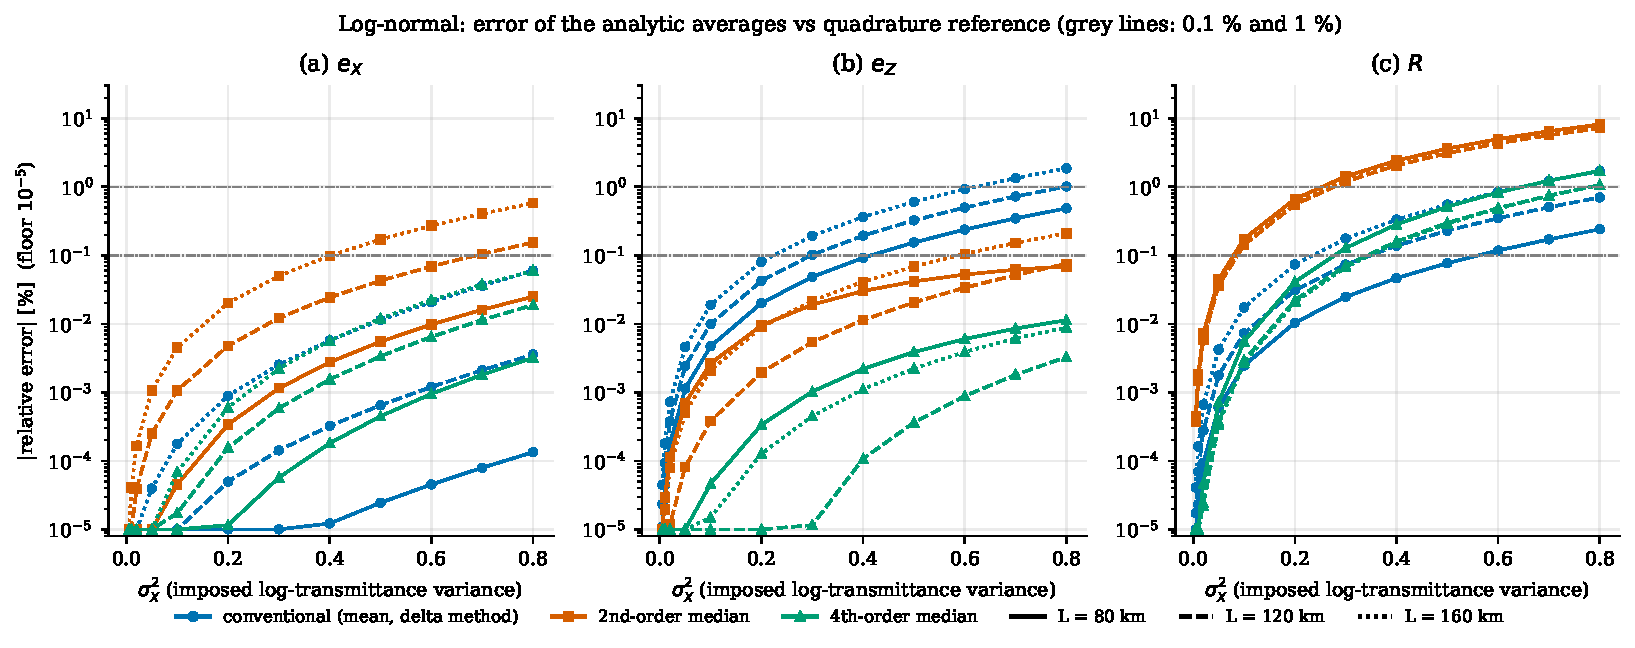
\includegraphics[width=\linewidth]{sens_fig_LN.pdf}\caption{Log-normal channel.}\label{fig:LN}\end{figure}
\begin{figure}[htbp]\centering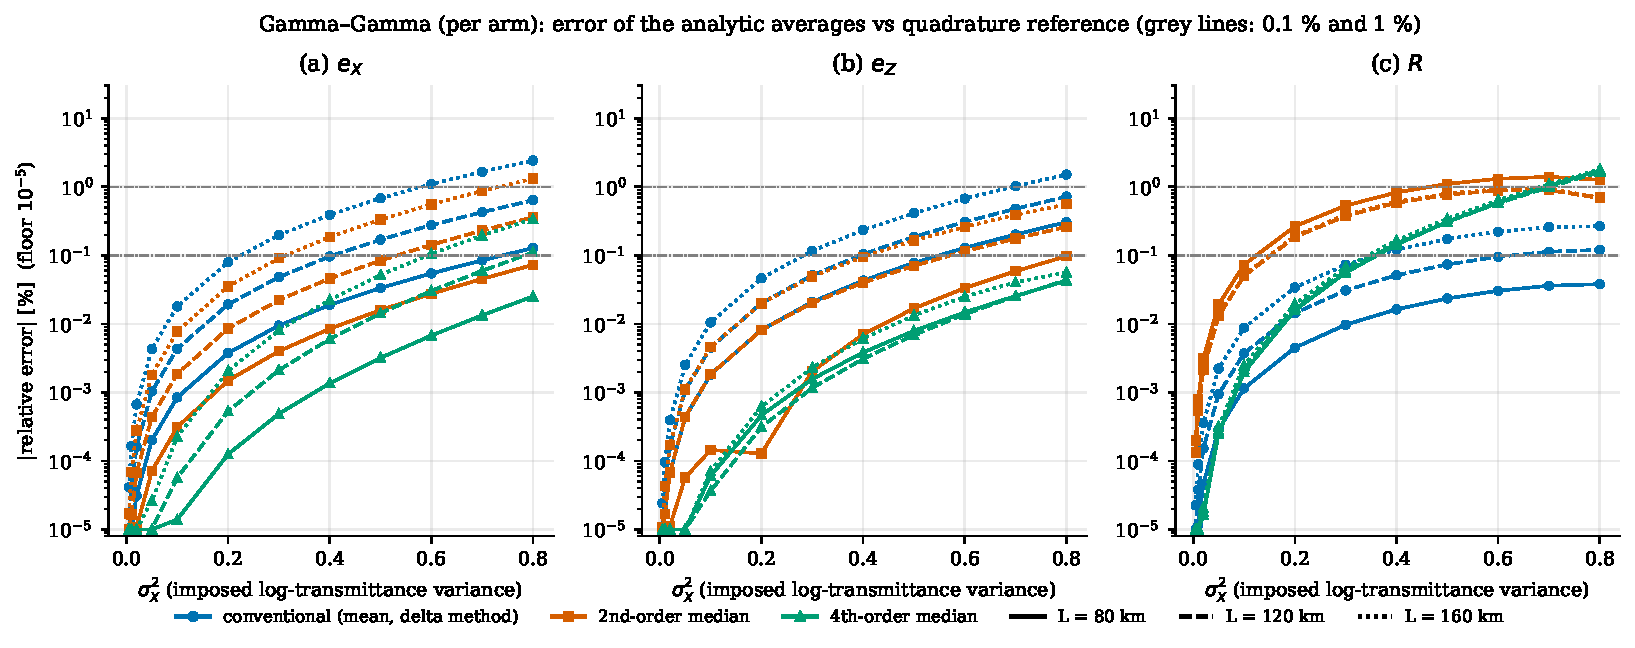
\includegraphics[width=\linewidth]{sens_fig_GG.pdf}\caption{Gamma--Gamma channel (per arm).}\label{fig:GG}\end{figure}
\begin{figure}[htbp]\centering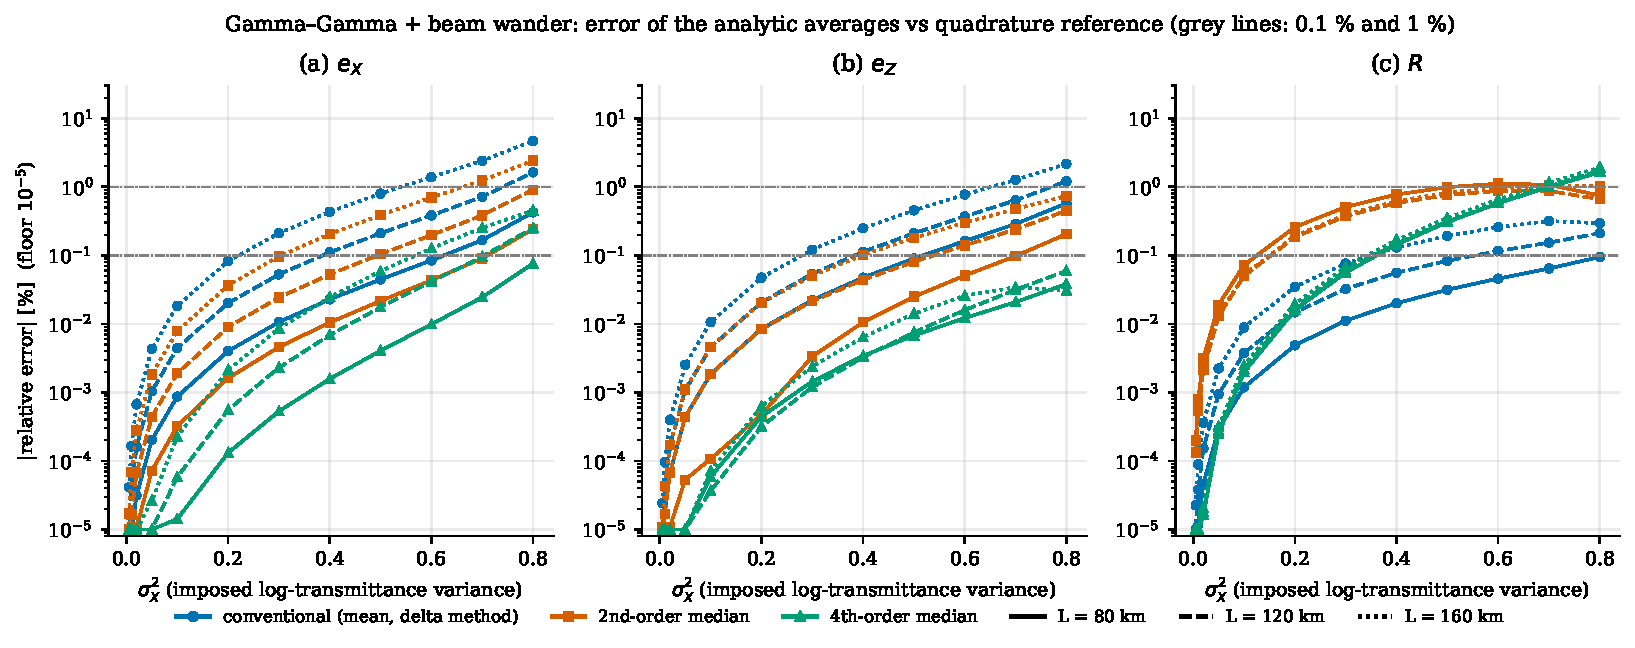
\includegraphics[width=\linewidth]{sens_fig_GGBB.pdf}\caption{Gamma--Gamma channel with beam wander (long-term beam broadening).}\label{fig:GGBB}\end{figure}

\section{Answers established by the data}
\paragraph{1. Does the approximation error increase with turbulence strength?}
Yes, in general. Of the $81$ (model, $L$, quantity, approximation) curves, $72$ increase monotonically in $|{\rm error}|$ over the grid and $9$ do not. The exceptions are the 2nd-order key-rate error of GG and GG+BB at all three distances (six curves; $|{\rm error}|$ peaks at $\sigma_X^2\approx0.6$--$0.7$ and then falls slightly, $1.40\to1.26\%$ at $80$~km for GG), the 2nd-order $e_Z$ of GG at $80$~km, and two small non-monotonicities at GG+BB, $160$~km (mean-approximation $R$, 4th-order $e_Z$). The size and the ranking of the errors depend on the quantity and on the distance (Table~\ref{tab:thr}, \ref{tab:thr2}): errors grow with distance at fixed $\sigma_X^2$ for $e_X$ and $e_Z$ in the GG models (e.g.\ mean-approximation $e_X$ error at $\sigma_X^2=0.8$: $0.13\%$, $0.64\%$, $2.4\%$ at $80,120,160$~km), because the operating point moves to a smaller $\eta_0$ where the error rates vary faster in $\ln\eta$. For $R$ the 4th-order error at $\sigma_X^2=0.8$ is nearly distance independent ($1.6$--$1.9\%$ in GG, $1.1$--$1.7\%$ in LN).

\paragraph{2. When does the 2nd-order approximation become insufficient for the key rate?}
Taking $0.1\%$ as the threshold for a ``precise'' value and $1\%$ for a ``usable'' one: the 2nd-order key-rate error exceeds $0.1\%$ at $\sigma_X^2\approx0.08$--$0.09$ for the log-normal channel and at $0.125$--$0.153$ for Gamma--Gamma, with or without beam wander; it exceeds $1\%$ at $\sigma_X^2\approx0.25$--$0.28$ (LN, all distances) and $0.47$ ($80$~km, GG), $0.51$ (GG+BB, $80$~km), and $0.65$ (GG+BB, $160$~km); for GG at $120$ and $160$~km and GG+BB at $120$~km it stays below $1\%$ up to $0.8$ (maxima $0.89$, $0.93$, $0.87\%$). The log-normal 2nd-order error reaches $7$--$8\%$ at $\sigma_X^2=0.8$. Conclusion: for the key rate the 2nd-order formula stops being accurate (to $0.1\%$) at $\sigma_X^2\approx0.1$, and (to $1\%$) at $\approx0.25$ in log-normal and around $0.5$ or not within the grid in Gamma--Gamma. At the realistic weak-class points ($\sigma_X^2=0.086$--$0.307$ LN, $c_2=0.084$--$0.258$ GG) the 2nd-order key-rate error, interpolated on the grid, is about $0.06$, $0.14$, $0.3\%$ (GG, $80,120,160$~km) and $0.13$, $0.5$, $1.3\%$ (LN).

\paragraph{3. Does the 4th-order approximation stay accurate over the tested range?}
It depends on the quantity.
\begin{itemize}
\item \emph{$e_X$ and $e_Z$:} yes. The 4th-order error stays below $0.46\%$ everywhere and below $0.1\%$ for all LN cases and for GG at $80$~km; its maximum is $0.45\%$ ($e_X$, GG+BB, $160$~km) and $0.06\%$ for $e_Z$. At $\sigma_X^2=0.8$ it is the best of the three approximations for $e_Z$ in every case and for $e_X$ in all GG and GG+BB cases and in LN at $160$~km (in LN at $80$ and $120$~km the mean approximation is marginally better for $e_X$, $\le0.004\%$).
\item \emph{$R$:} the error is bounded ($\le1.9\%$ for $\sigma_X^2\le0.8$) but it is \emph{not} uniformly small. It exceeds $0.1\%$ at $\sigma_X^2\approx0.28$--$0.36$ (LN $0.28$--$0.35$, GG and GG+BB $0.34$--$0.36$) and $1\%$ at $\approx0.65$--$0.78$ (LN $0.65$ at $80$~km and $0.78$ at $120$ and $160$~km; GG and GG+BB $0.68$--$0.70$). In Gamma--Gamma the 4th-order error \emph{overtakes} the 2nd-order one at $\sigma_X^2\approx0.7$ ($L=120,160$~km) and $0.8$ ($80$~km, GG and GG+BB): adding the $\Theta^3,\Theta^4$ terms no longer improves the result, i.e.\ the cumulant series is asymptotic and the third and fourth cumulants are no longer small corrections there. In the log-normal channel the 4th order is better than the 2nd throughout ($1.1$--$1.7\%$ against $7$--$8\%$ at $0.8$).
\item \emph{Surprise in the data:} the conventional mean-transmittance approximation is the \emph{most} accurate for $R$ at $\sigma_X^2=0.8$ in all GG and GG+BB cases ($\le0.30\%$) and in LN at $80$--$120$~km, although it is the worst for $e_X$ and $e_Z$. This is not evidence of a controlled expansion: at these operating points $R(\eta)$ is locally close to a power law ($d\ln R/d\ln\eta=1.05$--$1.13$ at $80$--$160$~km in the repository), for which the curvature correction in $\eta$ is small, and the delta-method error at $160$~km in the log-normal model already grows to $1.7\%$ at $\sigma_X^2=0.8$.
\end{itemize}

\paragraph{Beam wander.} In this controlled setting beam wander only shifts $\eta_0$ by $f_{\rm bb}$ (from $0.999$ to $0.09$--$0.18$ at $\sigma_X^2=0.8$); the key rate itself drops by up to a factor $3.6$ ($2.8$--$3.6$ at $\sigma_X^2=0.8$). The relative errors of $R$ differ from the plain GG case by at most $0.13$ percentage points. The errors of $e_X$ and $e_Z$ grow with the shift towards smaller $\eta_0$, mostly at $160$~km (mean approximation $e_X$ at $\sigma_X^2=0.8$: $2.4\to4.7\%$; 4th order: $0.34\to0.45\%$). The analytic formulas therefore keep their accuracy for the key rate with the beam-wander loss, and lose some for $e_X$ with the conventional approximation, \emph{provided} the shifted operating point stays on the smooth branch of the key-rate curve (all $\eta_m$ here do; $R(\eta_m)\ge6\times10^{-6}$).

\section{Limits}
Only $\sigma_X^2\le0.8$ was tested (the Gamma--Gamma maximum is $0.858$); log-normal behaviour above that, where the repository's validity limit $\sigma_R^2=1$ ($\sigma_X^2=0.5$) is already exceeded for $\sigma_X^2>0.5$, is not covered. The imposed values at fixed distance are a sensitivity device. Error values below $10^{-5}\%$ are plotted at a floor. Reproduction: \texttt{paper\_analysis/scripts/sensitivity\_study.py}, \texttt{sensitivity\_thresholds.py}, \texttt{sensitivity\_figures.py}, \texttt{sensitivity\_make\_tex.py} (they import the repository unchanged).
\end{document}
